\documentclass{article}

\usepackage{amsmath}
\usepackage{amssymb}
\usepackage{upgreek}
\usepackage{graphicx}
\usepackage[font={footnotesize,it}]{caption}
\usepackage[margin=0.5in]{geometry}
\setlength\parindent{0pt}

\begin{document}
\title{CPG formalization}
\author{Mahdi Khoramshahi}
\maketitle

Equations for one node in the network.

\begin{eqnarray}\label{eq:one_node}
	\dot \phi_i &=& \omega_{b} + \sum_{j \neq i} k_{ij} \sin \left( \phi_j - \phi_i - \tilde{\varphi}_{ij} \right ) + \zeta_i\\
	\Gamma_i    &=& A \cos(\phi_i)
\end{eqnarray}

where $\phi_i$ is the phase of \textit{i}th node, $k_{ij}$ and $\tilde{\varphi}_{ij}$ are coupling gain and desired phase lag between \textit{i}th and \textit{j}th node in the network. $\zeta_i$ is the input force for \textit{i}th which is determined by controller based on sensory information. 
Amplitude and frequency, $A$ and $\omega$ are equal for all nodes in the system. And finally, $\Gamma_i$ is the output of node and will be used as desired trajectory for \textit{i}th motor. \\

In our network, \textit{i} can be any of four actuators in our robot, namely \textit{front-right}, \textit{front-left}, \textit{hind-right}, and  \textit{hind-left} as shown in figure below, respectively node 1 to 4.

\begin{figure}[thpb]
	\centering
		\centering
		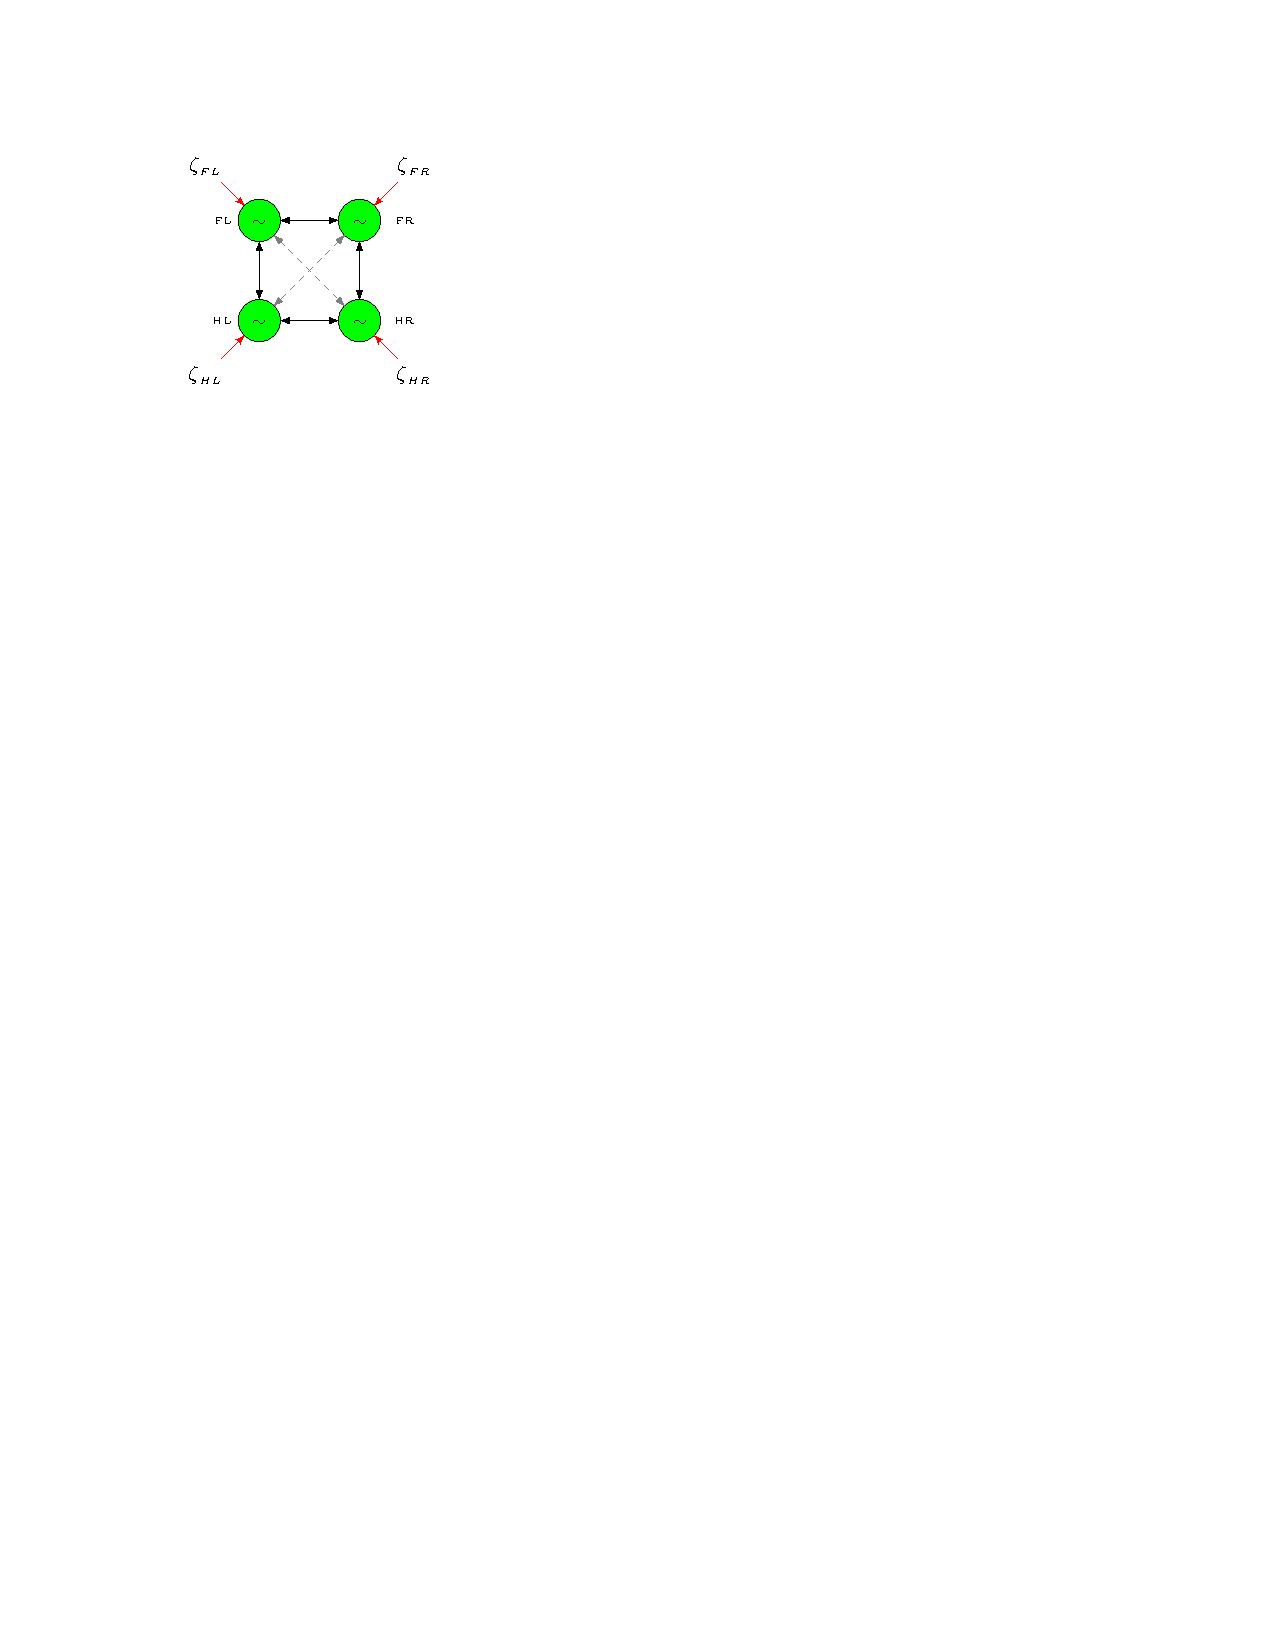
\includegraphics[scale = 0.95]{schema_cropped.pdf}
		\centering
		\caption{CPG network}
		\label{fig:CPG Network}

\end{figure}


In CPG network, $\varphi_{ij}$ determine the gait for robot. we chose the gait to be trot, therefore phase lags in matrix representation is:

	\[ \tilde{\Phi} = [\tilde{\varphi}_{ij}]=\left[ \begin{array}{rrrr}
	0    & \pi & \pi  & 0   \\
	-\pi & 0   & 0    & \pi  \\
	-\pi & 0   & 0    & \pi   \\
	0    & -\pi&-\pi  & 0 
	\end{array} \right].\]
	
This matrix is a skew-symmetry matrix because of phase lag property: $$\tilde{\varphi}_{ij} = - \tilde{\varphi}_{ji}$$  
As illustrated in Fig??, we are not using fully connected network. where dashed-grey line means coupling gain of zero.
we are using same coupling gain in the network, therefore matrix representation of coupling gains is:
 
 	\[ \upkappa = [k_{ij}]=\left[ \begin{array}{rrrr}
	0 & k & k & 0  \\
	k & 0 & 0 & k  \\
	k & 0 & 0 & k  \\
	0 & k & k & 0 
	\end{array} \right].\]

Differential equation of our CPG-Network is as follow:

\begin{eqnarray}\label{eq:cpg_net}
	\dot\phi_1&=&\omega_{b} + k\sin \left(\phi_2-\phi_1-\tilde{\varphi}_{12}\right)+k\sin\left(\phi_3-\phi_1-\tilde{\varphi}_{13}\right)+ \zeta_1\\
 	\dot\phi_2&=&\omega_{b} + k\sin \left(\phi_1-\phi_2-\tilde{\varphi}_{21}\right)+k\sin\left(\phi_4-\phi_2-\tilde{\varphi}_{24}\right)+ \zeta_2\\
 	\dot\phi_3&=&\omega_{b} + k\sin \left(\phi_1-\phi_3-\tilde{\varphi}_{31}\right)+k\sin\left(\phi_4-\phi_3-\tilde{\varphi}_{34}\right)+ \zeta_3\\
	\dot\phi_4&=&\omega_{b} + k\sin \left(\phi_2-\phi_4-\tilde{\varphi}_{42}\right)+k\sin\left(\phi_3-\phi_4-\tilde{\varphi}_{43}\right)+ \zeta_4
\end{eqnarray}

using following linear transformation $\varphi_{ij} = \phi_j - \phi_i - \tilde{\varphi}_{ij} $ and knowing the fact that $\dot{\tilde{\varphi}}_{ij} = 0$, and $\varphi_{ij} = - \varphi_{ji}$;  we will have our differential equation in phase lags coordination as follow:

\begin{eqnarray}\label{eq:cpg_net2}
	\dot\phi_1&=&\omega_{b} + k\sin \left(\varphi_{12}\right)+k\sin\left(\varphi_{13}\right)+ \zeta_1\\
 	\dot\phi_2&=&\omega_{b} + k\sin \left(\varphi_{21}\right)+k\sin\left(\varphi_{24}\right)+ \zeta_2\\
 	\dot\phi_3&=&\omega_{b} + k\sin \left(\varphi_{31}\right)+k\sin\left(\varphi_{34}\right)+ \zeta_3\\
	\dot\phi_4&=&\omega_{b} + k\sin \left(\varphi_{42}\right)+k\sin\left(\varphi_{43}\right)+ \zeta_4
\end{eqnarray}

\begin{eqnarray}\label{eq:cpg_net3}
	\dot\varphi_{12}&=& -2k\sin \left(\varphi_{12}\right)-k\sin\left(\varphi_{13}\right)+ k\sin\left(\varphi_{24}\right) + \zeta_2-\zeta_1\\
	\dot\varphi_{13}&=& -2k\sin \left(\varphi_{13}\right)-k\sin\left(\varphi_{12}\right)+ k\sin\left(\varphi_{34}\right) + \zeta_3-\zeta_1\\
	\dot\varphi_{24}&=& -2k\sin \left(\varphi_{24}\right)+k\sin\left(\varphi_{12}\right)- k\sin\left(\varphi_{34}\right) + \zeta_4-\zeta_2\\
	\dot\varphi_{34}&=& -2k\sin \left(\varphi_{34}\right)+k\sin\left(\varphi_{13}\right)- k\sin\left(\varphi_{24}\right) + \zeta_4-\zeta_3\\
\end{eqnarray}

Using ''\small{$\sin(\theta)=\theta$}'' approximation, linear autonomous can be expressed as follow:

  
  	\[ \dot{\Phi} = \frac{d}{dt} \Phi =\frac{d}{dt}
  	\left[\begin{array}{c}\varphi_{12} \\ \varphi_{13} \\ \varphi_{24} \\ \varphi_{34}\end{array}\right]
  	=k\left[ \begin{array}{rrrr}
	-2 & -1 &  1 &  0   \\
	-1 & -2 &  0 &  1  \\
	 1 &  0 & -2 & -1   \\
	 0 &  1 & -1 & -2 
	\end{array} \right] \Phi = \hat{A}\Phi.\] 
	
Eigenvalue of $\hat{A}$ are $-4k,-2k,-2k, 0$. We expected one zero eigenvalue-value due to the loop in our CPG network which cause linear relation between phase lag as follow: $$\varphi_{12} - \varphi_{13} + \varphi_{24} - \varphi_{34} = 0$$
negative eigenvalue shows that are our autonomous (unforced) system is locally asymptotically stable and it will converges to our desired phase lags. However, phase lag convergence will be effected by CPG inputs $\zeta_i$, but as we see from equations, phase lags are sensitive to mutual difference of $\zeta_i$. Therefor, closed-loop system should be design in way that minimize following costs:

\begin{eqnarray}\label{eq:one_node}
	\textit{Minimize    } \zeta_2-\zeta_1, \zeta_3-\zeta_1, \zeta_4-\zeta_2, \zeta_4-\zeta_3 
\end{eqnarray}
This minimization is equivalent to following minimization
\begin{eqnarray}\label{eq:one_node}
	\textit{Minimize    } \sigma_{\zeta} = \sum\limits_{i=1}^4 \left( \zeta_i - \bar{\zeta} \right)^2 \textit{, where } \bar{\zeta} = \frac{1}{4}\sum\limits_{i=1}^4\zeta_i.
\end{eqnarray}

Therefore, to provide achieve better converge to desired phase lags, it is very important to reduce variance of CPG inputs ($\zeta_i$). we will take advantage of dynamical null-space and we will define this constraint (Low variance input) as an task for controller.

\section*{Input Scheduling}
In order to control downward and upward motion separately, we split each CPG node input ($\zeta_i$) in two parts as follow:
\begin{eqnarray}\label{eq:one_node}
	\dot \phi_i &=& \omega_{b} + \sum_{j \neq i} k_{ij} \sin \left( \phi_j - \phi_i - \tilde{\varphi}_{ij} \right ) + \zeta_i^+ + \zeta_i^-\\
	\Gamma_i    &=& A \cos(\phi_i)
\end{eqnarray}

This input have the property $\zeta_i^+  \zeta_i^- = 0$, which means they cannot be active simultaneously. Upward and downward motions can be determined by checking the sign of $\sin(\phi)$ as shown in Fig??.

\begin{figure}[thpb]
	\centering
		\centering
		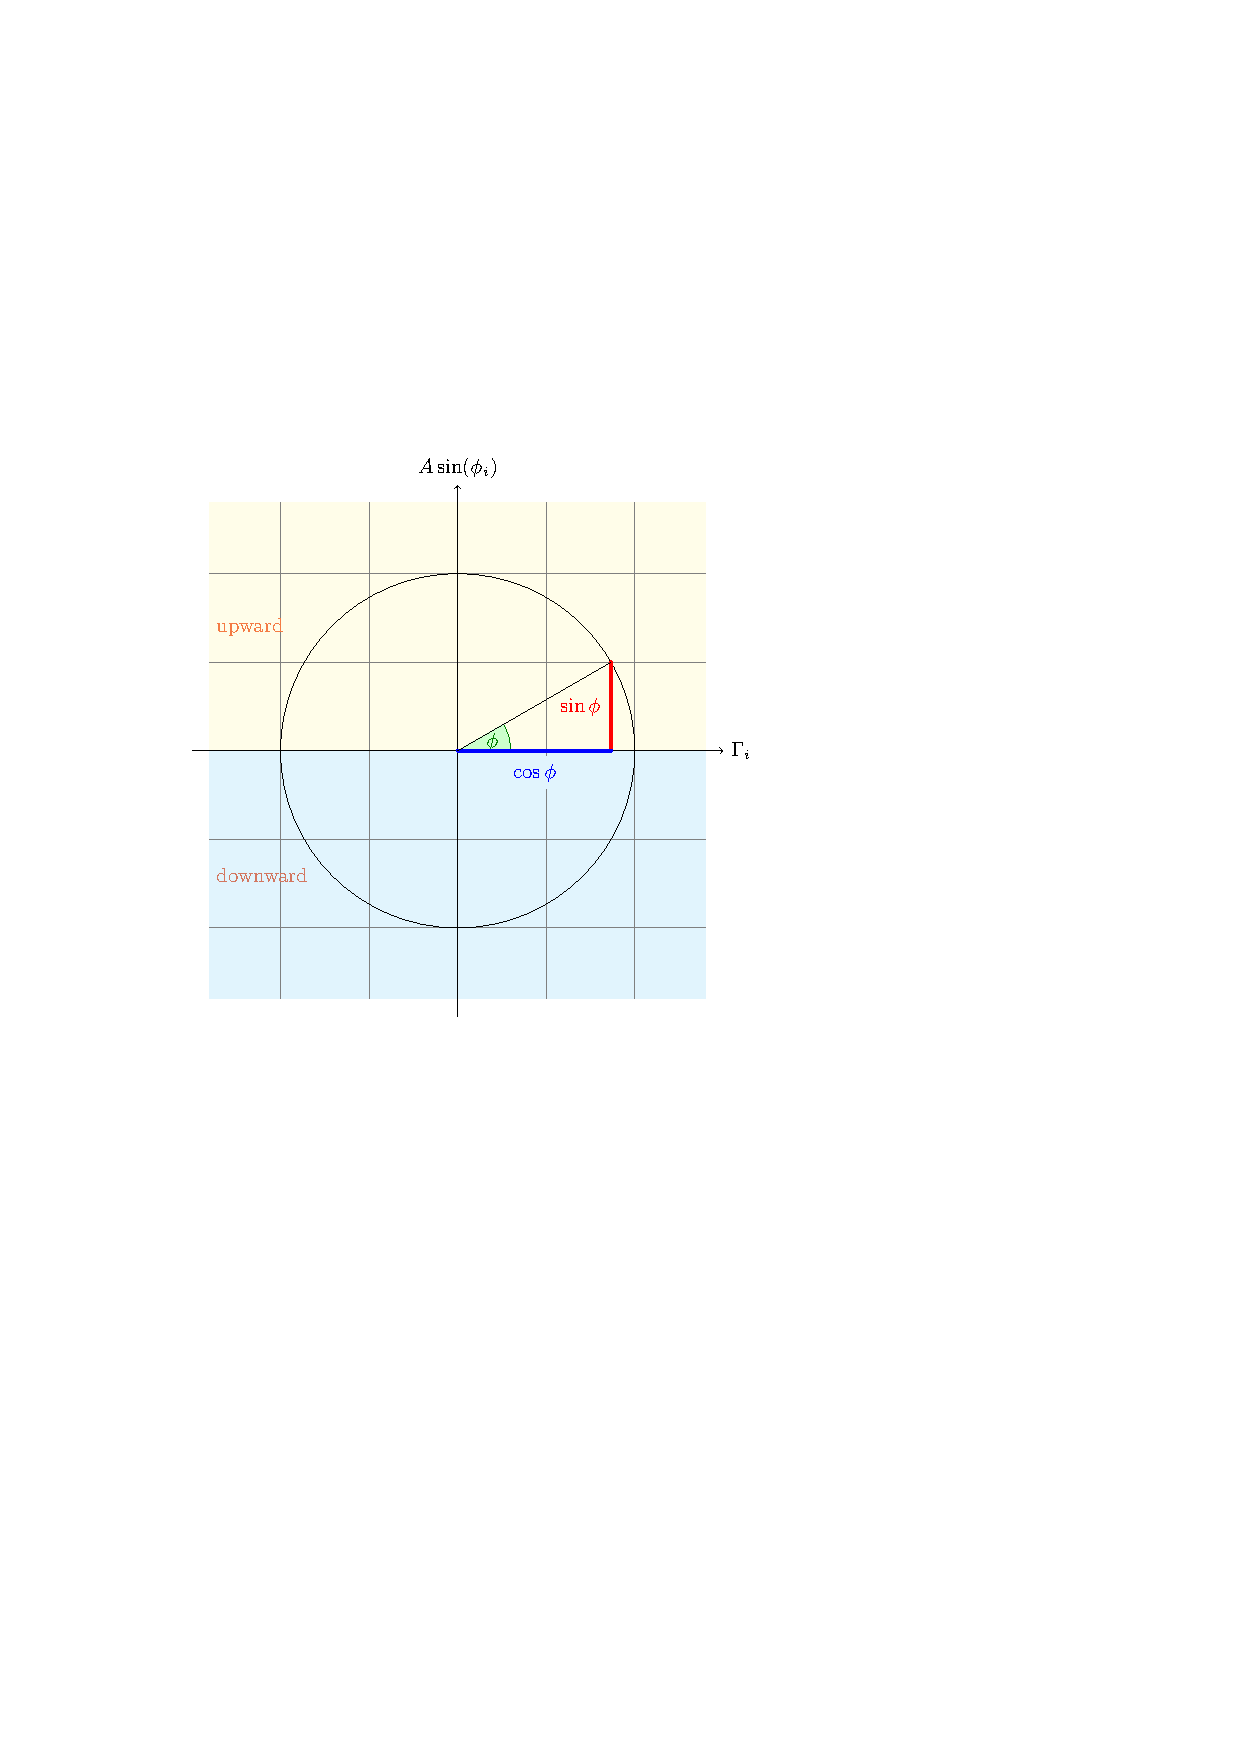
\includegraphics[scale = 0.7]{phase_plot_cropped.pdf}
		\centering
		\caption{phase}
		\label{fig:CPG Network}

\end{figure}



Splited CPG forces ($\omega^+$ , $\omega^-$) is provided by our controller. Thus, in order to build up our CPG force ($\zeta_i$), we will use: 

\begin{eqnarray}\label{eq:spliting}
	\zeta_i^+ &=& \frac{1}{2}[1+sign(\sin\phi)] \omega^+\\
	\zeta_i^- &=& \frac{1}{2}[1-sign(\sin\phi)] \omega^-\\
	\zeta_i &=& \zeta_i^+ + \zeta_i^-
\end{eqnarray}



\end{document}